% #############################################################################    % This is the MAIN DOCUMENT of the IST-UL-Project-Report TEMPLATE. 
% !TEX root = ./main.tex
% #############################################################################
% The document is automatically set for english or portuguese by just selecting
% the MAIN LANGUAGE in file 'IST-UL-Project-Report-Preamble.tex' 
% #############################################################################
% Version 1.0, October 2018
% BY: Prof. Rui Santos Cruz, rui.s.cruz@tecnico.ulisboa.pt
% #############################################################################
%  Set the document class
% ----------------------------------------------------------------------
\documentclass[12pt,a4paper,oneside]{report}
% -----------------------------------------------------------------------------
% The Preamble document contains all the necessary Packages for typesetting
% Modify it to suit your needs
% -----------------------------------------------------------------------------
% #############################################################################
% Preamble for IST-UL-Project-Report in English or Portuguese
% Required Packages and commands
% --> Please Choose the MAIN LANGUAGE for the Thesis in package BABEL (below)
% !TEX root = ./main.tex
% #############################################################################
% Version 1.0, October 2018
% BY: Prof. Rui Santos Cruz, rui.s.cruz@tecnico.ulisboa.pt
% #############################################################################
% -----------------------------------------------------------------------------
% PACKAGE ucs:
% -----------------------------------------------------------------------------
% The 'ucs' package provides support for using UTF-8 in LaTeX documents. 
% However in most situations it is not required.
\usepackage{ucs}
% -----------------------------------------------------------------------------
% PACKAGE utf8x:
% -----------------------------------------------------------------------------
% The 'utf8x' package contains support for using UTF-8 as input encoding. 
\usepackage[utf8x]{inputenc}
% -----------------------------------------------------------------------------
% PACKAGE babel:
% -----------------------------------------------------------------------------
% The 'babel' package may correct some hyphenation issues of LaTeX. 
% Select your MAIN LANGUAGE for the Thesis with the 'main=' option.
% 
\usepackage[main=english,portuguese]{babel}
% -----------------------------------------------------------------------------
% PACKAGE iflang:
% -----------------------------------------------------------------------------
% The 'iflang' package is used to help determine the language being used. 
\usepackage{iflang}

% ----------------------------------------------------------------------
% Define default and cover page fonts.
% ----------------------------------------------------------------------
% Use Arial font as default
%
\renewcommand{\rmdefault}{phv}
\renewcommand{\sfdefault}{phv}
\def\FontLn{% 16 pt normal
  \usefont{T1}{phv}{m}{n}\fontsize{16pt}{16pt}\selectfont}
\def\FontLb{% 16 pt bold
  \usefont{T1}{phv}{b}{n}\fontsize{16pt}{16pt}\selectfont}
\def\FontMn{% 14 pt normal
  \usefont{T1}{phv}{m}{n}\fontsize{14pt}{14pt}\selectfont}
\def\FontMb{% 14 pt bold
  \usefont{T1}{phv}{b}{n}\fontsize{14pt}{14pt}\selectfont}
\def\FontSn{% 12 pt normal
  \usefont{T1}{phv}{m}{n}\fontsize{12pt}{12pt}\selectfont}
% ----------------------------------------------------------------------
% Define page margins and line spacing.
% ----------------------------------------------------------------------
% > set the page margins (2.5cm minimum in every side, as per IST rules)
%
\usepackage{geometry}	
\geometry{verbose,tmargin=2.5cm,bmargin=2.5cm,lmargin=2.5cm,rmargin=2.5cm}
%
% > allow setting line spacing (line spacing of 1.5, as per IST rules)
%
\usepackage{setspace}
\renewcommand{\baselinestretch}{1.5}
% ----------------------------------------------------------------------
% Include external packages.
\usepackage{graphicx}
\usepackage{amsmath}  % AMS mathematical facilities for LaTeX.
\usepackage{amsthm}   % Typesetting theorems (AMS style).
\usepackage{amsfonts} % 
\usepackage{subfigure}
\usepackage{subfigmat}
\usepackage{dcolumn}
\newcolumntype{d}{D{.}{.}{-1}} % column aligned by the point separator '.'
\newcolumntype{e}{D{E}{E}{-1}} % column aligned by the exponent 'E'
\usepackage[pdftex]{hyperref} % enhance documents that are to be
                              % output as HTML and PDF
\hypersetup{colorlinks,       % color text of links and anchors,
                              % eliminates borders around links
            linkcolor=blue,  % color for normal internal links
            anchorcolor=black,% color for anchor text
            citecolor=cyan,  % color for bibliographical citations
            filecolor=black,  % color for URLs which open local files
            menucolor=black,  % color for Acrobat menu items
            urlcolor=teal,   % color for linked URLs
	        bookmarksopen=true,    % don't expand bookmarks
	        bookmarksnumbered=true, % number bookmarks
            }
\usepackage[figure,table]{hypcap}
\usepackage[format=hang,labelfont=bf,font=small]{caption} 
\captionsetup[table]{skip=10pt}
\usepackage{cite}
\usepackage[printonlyused]{acronym}
\usepackage{lipsum}

% -----------------------------------------------------------------------------
% PACKAGE Cleveref:
% -----------------------------------------------------------------------------
% Clever Referencing of document parts
% Note: portuguese is supported through "brazilian" option
\usepackage[\IfLanguageName{english}{english}{brazilian}]{cleveref}
% -----------------------------------------------------------------------------
% PACKAGES xcolor, color
% -----------------------------------------------------------------------------
% These packages are required for list code snippets.
\usepackage{xcolor}
\usepackage{color}
% The following special color definitions are used in the IST Thesis
\definecolor{forestgreen}{RGB}{34,139,34}
\definecolor{orangered}{RGB}{239,134,64}
\definecolor{lightred}{rgb}{1,0.4,0.5}
\definecolor{orange}{rgb}{1,0.45,0.13}	
\definecolor{darkblue}{rgb}{0.0,0.0,0.6}
\definecolor{lightblue}{rgb}{0.1,0.57,0.7}
\definecolor{gray}{rgb}{0.4,0.4,0.4}
\definecolor{lightgray}{rgb}{0.95, 0.95, 0.95}
\definecolor{darkgray}{rgb}{0.4, 0.4, 0.4}
\definecolor{editorGray}{rgb}{0.95, 0.95, 0.95}
\definecolor{editorOcher}{rgb}{1, 0.5, 0} % #FF7F00 -> rgb(239, 169, 0)
\definecolor{chaptergrey}{rgb}{0.6,0.6,0.6}
\definecolor{editorGreen}{rgb}{0, 0.5, 0} % #007C00 -> rgb(0, 124, 0)
\definecolor{olive}{rgb}{0.17,0.59,0.20}
\definecolor{brown}{rgb}{0.69,0.31,0.31}
\definecolor{purple}{rgb}{0.38,0.18,0.81}




\usepackage{listings}
\lstset{escapeinside={<@}{@>}}
\usepackage{minted}

\lstdefinestyle{commandline} {%
language={[WinXP]command.com},
breaklines=true,
%aboveskip=\baselineskip,
belowskip=\baselineskip,
showstringspaces=false,
backgroundcolor=\color{black},
basicstyle=\small\color{white}\ttfamily
showstringspaces=false,
keywordstyle=\color{cyan}\bfseries,
stringstyle=\color{gray}\ttfamily,
commentstyle=\color{green}\itshape,
moredelim=[s][\color{yellow}\bfseries]{C:}{\>}
}

\lstdefinestyle{Bash} {%
language=bash,
breaklines=true,
belowskip=\baselineskip,
backgroundcolor=\color{lightgray},
showstringspaces=false,
keywordstyle=\color{black}\bfseries,
basicstyle=\small\color{black}\ttfamily,
stringstyle=\color{editorOcher}\ttfamily,
commentstyle=\color{brown}\itshape,
otherkeywords={xcode-select, mkdir,rm},
moredelim=[s][\color{darkblue}]{~$},
literate={~} {$\sim$}{1}
}

\lstdefinestyle{Rubytext} {%
language=Ruby,
breaklines=true,
belowskip=\baselineskip,
basicstyle=\small\ttfamily\color{black},
backgroundcolor=\color{lightgray},
showstringspaces=false,
commentstyle = \ttfamily\color{red},
keywordstyle=\ttfamily\color{blue},
stringstyle=\color{orange}
}
\lstset{escapeinside={<@}{@>}}

\lstdefinestyle{py} {%
	language=python,
	literate=%
	*{0}{{{\color{red}0}}}1
	{1}{{{\color{red}1}}}1
	{2}{{{\color{red}2}}}1
	{3}{{{\color{red}3}}}1
	{4}{{{\color{red}4}}}1
	{5}{{{\color{red}5}}}1
	{6}{{{\color{red}6}}}1
	{7}{{{\color{red}7}}}1
	{8}{{{\color{red}8}}}1
	{9}{{{\color{red}9}}}1,
	basicstyle=\small\ttfamily,
	numbers=left,
	% numberstyle=\tiny,
	% stepnumber=2,
	numbersep=5pt,
	tabsize=4,
	extendedchars=true,
	breaklines=true,
	keywordstyle=\color{blue}\bfseries,
	frame=b,
	commentstyle=\color{brown}\itshape,
	stringstyle=\color{editorOcher}\ttfamily,
	showspaces=false,
	showtabs=false,
	xleftmargin=17pt,
	framexleftmargin=17pt,
	framexrightmargin=5pt,
	framexbottommargin=4pt,
	backgroundcolor=\color{lightgray},
	showstringspaces=false,
}










% DEFINE COMMAND FOR: Acronyms listing Title depending on language
\newcommand{\tlangAcronyms}{\IfLanguageName{english}{Acronyms}{Acr\'onimos}}
% DEFINE COMMAND FOR: Degree Title depending on language
\newcommand{\tlangDegree}{\IfLanguageName{english}{Information Systems and Computer Engineering}{Engenharia Informática e de Computadores}}
% DEFINE COMMAND FOR: Course Title depending on language
\newcommand{\tlangCourse}{\IfLanguageName{english}{Management and Administration of IT Infrastrutures and Services}{Administração e Gestão de Infraestruturas e Serviços de IT}}
%%%%%%%%%%%%%%%%%%%%%%%%%%%%%%%%%%%%%%%%%%%%%%%%%%%%%%%%%%%%%%%%%%%%%%%%



% #############################################################################
\begin{document}
% Set plain page style (no headers, footer with centered page number)
\pagestyle{plain}
% Set roman numbering (i,ii,...) before the start of chapters
\pagenumbering{roman}
% ----------------------------------------------------------------------------
%  Cover page
% #############################################################################     % This is the FRONT COVER of the IST-UL-Project-Report TEMPLATE. 
% !TEX root = ./main.tex
% #############################################################################
% Version 1.0, October 2018
% BY: Prof. Rui Santos Cruz, rui.s.cruz@tecnico.ulisboa.pt
% #############################################################################
% #############################################################################
% DO NOT CHANGE THE FOLLOWING 4 LINES
\thispagestyle {empty}

\includegraphics[width=5cm]{./pictures/IST_A_RGB_POS.png}
\begin{center}
\vspace{5.0cm}
% #############################################################################
% #############################################################################
%
% INSERT THE TITLE OF THE PROJECT HERE
{\FontLb RocketChat \& Monitoring deployed in Cloud} \\
\vspace{0.2cm}
%
% INSERT THE SUBTITLE OF THE REPORT HERE
{\FontMn A Scalable Microservices-based Web Application in a Public Cloud} \\
\vspace{1.0cm}
{\FontLn \tlangCourse} \\
\vspace*{1.0cm}
\begin{center}
\begin{tabular}{r@{~}l l}
    \multicolumn{3}{c}{\bfseries\textbf{ }} \\
    % INSERT YOUR TEAM NUMBER HERE
    & \textbf{Team nr.}: & 06 \\
    % INSERT IDs and NAMES of STUDENTS 
    & 98678: & Bruno Freitas \\
    & 98844: & André Barrocas \\
    & 102108: & Ricardo Ribeiro \\ % Comment if not necessary
    %& Student-ID-4: & Student-Full-Name-4 \\ % Comment if not necessary
    %& Student-ID-5: & Student-Full-Name-5 \\ % Comment if not necessary
\end{tabular}
\end{center}
\vspace*{2.0cm}
{\FontMb \tlangDegree} \\
{\FontMb IST-ALAMEDA} \\
\vspace{1.5cm}
{\FontMb 2021/2022} \\
\end{center}
\cleardoublepage
% ----------------------------------------------------------------------------
%  Table of contents, list of tables, list of figures and nomenclature
% ----------------------------------------------------------------------------
\tableofcontents
\clearpage 
\begingroup 
    \let\clearpage\relax
    \let\cleardoublepage\relax
    \let\cleardoublepage\relax
% List of tables
%\listoftables
% Add entry in the table of contents as section
%\addcontentsline{toc}{section}{\listtablename}
% List of figures
\listoffigures
% Add entry in the table of contents as section
\addcontentsline{toc}{section}{\listfigurename}
\endgroup
% --------------------------------------------------------------------------
%  acronyms DEFINE YOUR ACRONYMS HERE
% --------------------------------------------------------------------------
\chapter*{\tlangAcronyms}
\begin{acronym}[NGOSS]
	\acro{GCP}{Google Cloud Platform}
	\acro{AWS}{Amazon web Services}
	\acro{mongoDB}{Mongo database}
	\acro{JSON}{JavaScript Object Notation}
	\acro{VM}{Virtual Machine}
	\acro{K8s}{Kubernetes}
	\acro{DNS}{Domain Name System}
\end{acronym}
% Set arabic numbering (1,2,...) after preface
\setcounter{page}{1}
\pagenumbering{arabic}
% #############################################################################
%
%                           BEGIN MAIN DOCUMENT BODY
%
% #############################################################################
\chapter{Executive Summary}
\label{chapter:introduction}
The goal of this work is to show an example on how to deploy and provision tiered (frontend, backend) Microservices-based containerized Web Application on a Public Cloud provider, such as \ac{GCP} or \ac{AWS}, using automation tools such as Terraform, Ansible, Pulumi, as well as implementing instrumentation on the applications, services and infrastructure components of the solution, to allow monitoring and logging features by using tools such as Prometheus, Fluentd, etc.

This work studies the RocketChat which is an open-source platform for team collaboration, allowing live chat, direct message and group messages, upload the images and, other interesting features. \cite{rocketchat} It is written in full-stack JavaScript and uses the \ac{mongoDB}. Mongo is a NoSQL database, using JSON-like documents as schema. \cite{mongodb} To complete a monitoring system it is also implemented. To make the monitoring, the Grafana and Prometheus were used. Grafana is a open source analytics and interactive visualization web application that provides charts, graphs, and alerts for the web. \cite{grafana} The purpose of Grafana dashboards allows the users to better understand the metrics. Prometheus is an open-source event monitoring and alerting tool that records real-time metrics, with flexible queries and real-time alerting. \cite{prometheus}

This report starts by talking about the System Architecture \ref{chapter:sys-architecture}, and approaching its requirements and constraints. The next chapter \ref{chapter:deployment} shows how to deploy the project and some images of the project running. In the Versioning Chapter \ref{chapter:versioning} how the system versions were managed will be explained and for the last part, which is the Evolution Chapter \ref{chapter:work-evol}, it approaches the extra steps the group has taken in order to achieve the best solution possible in the time given (for example, it is approached the previous version of the project, the docker-compose version).

There is also a Video related to this project, stating how to deploy and giving an overview oh the work done. This video can be found in the following link: \url{https://www.youtube.com/watch?v=e5jRSE9jek8}

\cleardoublepage
% #############################################################################
\chapter{System Architecture}
\label{chapter:sys-architecture}
\begin{figure}[h]
    \centering
    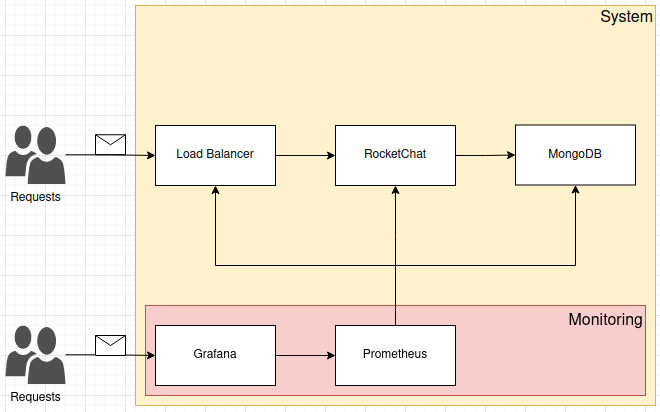
\includegraphics[width=1.0\textwidth]{./pictures/overview-system-architecture.png}
    \caption{Overview System Architecture}
    \label{fig:overview-sys-architecture}
\end{figure}

By the Figure \ref{fig:overview-sys-architecture}, it is possible to see in a generic way how the system is composed. The system is used to satisfy two use cases, the monitoring use case and the "normal" web service use case. The first one is related to how a user can watch all the metrics. The second one is related to how a user can use the web service application.

\begin{itemize}
    \item \textbf{Monitoring use case:} The user will access the Grafana dashboard to see the metric collected. Grafana will interact with Prometheus who is responsible to collect the metrics related with all the components of the system (in the next section \ref{section:analysis} it will be explained that the system will be deployed as a cluster and the metrics collected will be from the cluster itself).
    \item \textbf{Web Service Application use case:} The user will access the frontend web page of RocketChat to use the application. The application's frontend will talk with \ac{mongoDB} to handle the database operations. The load balancer says that the requests from users will be distributed to the RocketChat Servers (more than one to support more users with better performance)
\end{itemize}

% #############################################################################
\section{Analysis}
\label{section:analysis}
The system will be built on top of \ac{K8s} in order to satisfy the system requirements. 

\begin{figure}[htb]
    \centering
    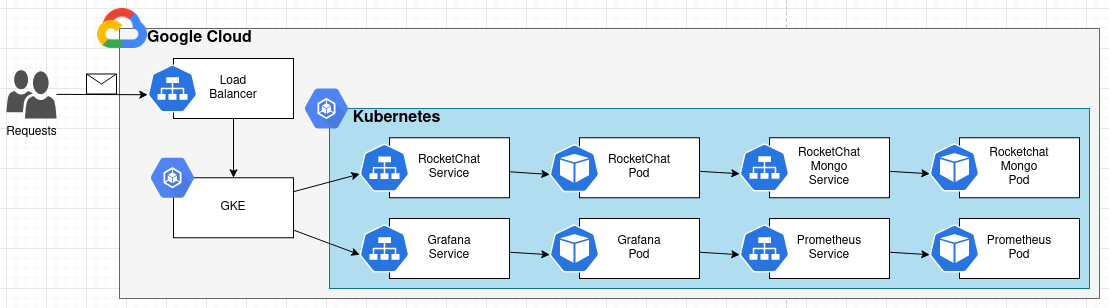
\includegraphics[width=1.0\textwidth]{./pictures/system_architecture_k8s.png}
    \caption{System Architecture in Kubernetes}
    \label{fig:sys-architecture-k8s}
\end{figure}

As it can be seen in the Figure \ref{fig:sys-architecture-k8s}, the \ac{K8s} environment is composed with several objects:
\begin{itemize}
    \item \textbf{RocketChat Pods} to handle the requests from the client (RocketChat servers). The Pod contains a RocketChat container inside of it, and the port 3000 is exposed to be possible to contact the RocketChat app;
    \item \textbf{RocketChat Service} to load-balance the client requests for the RocketChat Pods. The Service type is LoadBalancer, provisioning a load balancer for the service. It is exposing port 3000 to outside and forwards traffic to port 3000 to RocketChat Pods;
    \item \textbf{RocketChat Mongo Pods} to handle the requests from RocketChat servers and persist the data into the database, persisted in a volume; The Pod contains the RocketChat-Mongo container responsible for what has been written behind, and a second container called "rocketchat-mongo-sidecar" which is the sidecar container that will automatically configure the new Mongo nodes to join the replica set;
    \item \textbf{RocketChat Mongo Service} to forward the traffic to Mongo Pods. The Service is a headless service so, there is no load balancing or proxying done. It defines the selector so, endpoint records will be created in the API, and the \ac{DNS} returns A records (IP addresses) that point directly to the Pods backing the Service;
    \item \textbf{Grafana Pods} to handle the requests for monitoring purposes. The Pod contains a Grafana container inside of it, exposing the port 3000 to be possible to contact the Grafana app;
    \item \textbf{Grafana Service} to load-balance the client requests for Grafana Pods. The Service type is LoadBalancer, provisioning a load balancer for the service. It is exposing port 3000 to outside and forwards traffic to port 3000 to Grafana Pods;
    \item \textbf{Prometheus Pods} that collect metrics about the cluster and its resources. The Pod contains a Prometheus container inside of it, exposing the port 9090 to be possible to contact the Prometheus app;
    \item \textbf{Prometheus Service} to load-balance the client requests for the Prometheus Pods. The Service type is LoadBalancer, provisioning a load balancer for the service. It is exposing port 9090 to outside and forwards traffic to port 9090 to Prometheus Pods.
\end{itemize}

There is two important factor to notice here. The first one is that there is two \ac{K8s} namespaces which organizes the cluster into virtual sub-clusters leading to better management by different teams in a real world environment. With this in mind, an \textbf{application} namespace was created, containing the RocketChat Server and Mongo Pods and their Services. The other name space is called \textbf{istio-system} and contains all resources related to monitoring, the Grafana and Prometheus Pods, their Services and other important resources. The second important factor is the fact that all these Pods can be scaled up or scaled down depending on the need.

% #############################################################################
%\newpage
\subsection{Built With}
\label{section:built-with}
\begin{itemize}
    \item \textbf{Vagrant} (\url{https://www.vagrantup.com/}) - Vagrant provides the same, easy workflow regardless of your role as a developer, operator, or designer.
    \item \textbf{Terraform} (\url{https://www.terraform.io/}) - Terraform is an open-source infrastructure as code software tool that provides a consistent CLI workflow to manage hundreds of cloud services.
    \item \textbf{Docker} (\url{https://docker.com/}) - Docker is the \#1 most wanted and #2 most loved developer tool, and helps millions of developers build, share and run any app, anywhere-on-prem or in the cloud.
    \item \textbf{Google Cloud Platform} (\url{https://cloud.google.com}) - Reliable and high performance cloud platform from Google.
    \item \textbf{Kubernetes} (\url{https://kubernetes.io}) - Kubernetes is an open-source container-orchestration system for automating computer application deployment, scaling, and management.
\end{itemize}

The following technologies were also used in the docker-compose version of the project (previous version - more information in Evolution Chapter \ref{chapter:work-evol}):
\begin{itemize}
    \item \textbf{Ansible} (\url{https://www.ansible.com/}) - Ansible is an open source community project sponsored by Red Hat, it's the simplest way to automate IT.
    \item \textbf{Docker Compose} (\url{https://docs.docker.com/compose/}) - Compose is a tool for defining and running multi-container Docker applications. With Compose, you use a YAML file to configure your application's services.
\end{itemize}

% #############################################################################
\subsection{Requirements}
\label{section:requirements}
\paragraph{The Requirements to Run the Application} are the following software:
\begin{description}
\item[R01] Vagrant (latest);
\item[R02] Virtualbox (latest).
\end{description}

To confirm that the software is installed, type in a terminal the following commands:
\begin{lstlisting} [style=Bash]
$ vagrant --version
$ vboxmanage --version
\end{lstlisting}

Vagrant is necessary to create the \textbf{management machine}. This is done with a Vagrantfile that uses a Virtualbox provider (this Vagrant file is not prepared to run on systems with architecture ARM arch64, namely Apple Silicon M1 computers - to run this on a machine with these characteristics, another provider such as Docker must be used).

It is also a requirement to have a \textbf{\ac{GCP} account}. With this it is possible to create a project, enable the API (see the note below to further information) and then it is needed to download the credentials.json to the terraform folder (to authenticate the project).

\textbf{NOTE:} It is needed to ENABLE APIs AND SERVICES for the Project, by choosing in the Google Cloud Console API & services and next selecting the Dashboard, where it is possible to see a button on the top menu for enabling those services. Then enable \textbf{Kubernetes Engine API}.

\paragraph{The Requirements for the System} are:
\begin{description}
\item[R01] \label{itm:r01} Easy and Automatic Deployment;
\item[R02] \label{itm:r02} Scalability;
\item[R03] \label{itm:r03} Portability;
\item[R04] \label{itm:r04} Flexibility.
\end{description}

For the \textbf{R01} requirement, the system is deployed using Terraform. It is only needed to run the commands described in the Deployment Chapter \ref{chapter:deployment} and everything will be deployed. For the \textbf{R02}, \textbf{R03} and \textbf{R04} requirements, the system is deployed on top of Kubernetes which although it is more complex, it allows for autoscaling, it is flexible and portable, meaning it works in any type of underlying infrastructure and it can be used on many different infrastructure and environment configurations.

% #############################################################################
\subsection{Constraints}
\label{section:constraints}
Here are the Constraints for the System:
\begin{description}
\item[C01] The configuration of MONGO\_URL and MONGO\_OPLOG\_URL for the RocketChat-Server Pods need to be written manually.
\end{description}

Scaling up the \ac{mongoDB} it is automatic and the new Pods will automatically join the replica-set of \ac{mongoDB}. This happens because of the sidecar container used, explained in the Analysis Section \ref{section:analysis}. The \textbf{C01} constraints exists because the RocketChat application needs two environment variables called MONGO\_URL and \newline MONGO\_OPLOG\_URL \cite{rocketchat-create-docker-container}. These variables need to declare how to access the \ac{mongoDB} nodes of the replica-set. For example, let's say that a new fifth Pod of RocketChat Mongo was added to the replica-set. Now, it is needed to add to MONGO\_URL and MONGO\_OPLOG\_URL how to get to this new Pod, by adding the DNS name of this new Pod, for this example would be something like "rocketchat-mongo-5.rocketchat-mongo.application" ($<$pod-name$>$.$<$service-name$>$.$<$namespace$>$).

All this research is supported by the Kubernetes documentation on how to Run MongoDB on Kubernetes with StatefulSets document \cite{running-mongodb-on-kubernetes} that says the following: "Include the two new nodes in your connection string URI and you are good to go. Too easy!"

% #############################################################################
\subsection{Project Structure}
\label{section:proj-structure}
\begin{verbatim}
|- Vagrantfile
|- bootstrap-mgmt.sh
|- docs
|- docker-compose-version
\- tools
    \- terraform
        |- agisit-2021-rocketchat-06.json
        \- cluster
            |- gcp-gke-main.tf
            |- gcp-gke-provider.tf
            |- terraform.tfvars
            |- gcp_gke
                |	\- gcp-gke-cluster.tf
            \- gcp_k8s
                |- monitoring
                |   |- grafana.yaml
                |   \- prometheus.yaml
                |- k8s-istio.tf
                |- k8s-monitoring.tf
                |- k8s-namespaces.tf
                |- k8s-pods.tf
                |- k8s-provider.tf
                |- k8s-services.tf
                \- k8s-variables.tf
\end{verbatim}
\begin{itemize}
    \item At the root there is the `Vagrantfile` needed to create the management VM (`mgmt`). For this, the `bootstrap-mgmt.sh` script will be executed and, the goal of this script to install the necessary software, or in other words, prepare the management machine. The management machine will be used to do all the operations of the project;
    \item The `docs` folder contains the reports from all checkpoints and images;
    \item the `docker-compose-version` contains the previous checkpoints' implementation (more information in the Evolution Chapter \ref{chapter:work-evol});
    \item The `tools` folder contains all the project's infrastructure/services files that will be deployed with the help of our `mgmt` VM. Inside of this folder there is:
    \begin{itemize}
        \item The `terraform` folder to provision the infrastructure. Here we have the following folders and files:
        \subitem The json file with the credentials to be used in the deployment of the cluster. (you should change this file to the credentials of your project!);
        \subitem The folder `cluster` that contains everything used to deploy the entire cluster infrastructure:
        \begin{itemize}
            \item `gcp-gke-main.tf`, defines the modules used for the deployment and provisioning;
            \item `gcp-gke-provider.tf`, defines the provider to be used;
            \item `terraform.tfvars`, defines some variables used with the Terraform files;
            \item `gcp\_gke`, folder for the cluster definition file;
                \subitem `gcp-gke-cluster.tf`, defines the cluster as well as outputs certain values.
            \item `gcp\_k8s`, folder containing the Terraform files defining the pods, services, namespaces and other resources needed.
                \subitem the `monitoring` folder with :
                    \begin{itemize}
                        \item `grafana.yaml`, entire configuration file for the Grafana system.
                        \item `prometheus.yaml`, entire configuration file for the Prometheus system.
                    \end{itemize}
                \subitem `k8s-istio.tf`, ISTIO Service Mesh deployment via helm charts.
                \subitem `k8s-monitoring.tf`, deploys Grafana and Prometheus referring to the yaml files in folder monitoring
                \subitem `k8s-namespaces.tf`, defines namespaces used.
                \subitem `k8s-pods.tf`, defines the Pods to be deployed.
                \subitem `k8s-provider.tf`, defines the providers that Terraform needs and certain configurations for each of them.
                \subitem `k8s-services.tf`, defines the Pods' Services.
                \subitem `k8s-variables.tf`, variables to be used that are obtained after the provisioning of the cluster.
        \end{itemize}
    \end{itemize}
\end{itemize}

\cleardoublepage
% #############################################################################
\chapter{Deployment}
\label{chapter:deployment}
This project was design to have a easy deployment. So, the first thing to do is to go to the project directory and run the following commands to put up and connect to the `mgmt` - Management \ac{VM} (bastion):

\begin{lstlisting} [style=Bash]
$ vagrant up
$ vagrant ssh mgmt
\end{lstlisting}

After this, inside the `mgmt`, run the following command to authenticate in the \ac{GCP} (it will give a link, open it on a browser, login in with an IST account, copy the response code and past the verification code in the command line):

\begin{lstlisting} [style=Bash]
vagrant@mgmt:~$ gcloud auth login
\end{lstlisting}

Then, inside the `mgmt`, let's create the infrastructure by running the commands (first will initialize Terraform, in order to satisfy some plugin requirements; then it will create a plan and create the infrastructure by running apply):

\begin{lstlisting} [style=Bash]
vagrant@mgmt:~/tools/terraform/cluster$ terraform init
vagrant@mgmt:~/tools/terraform/cluster$ terraform plan
vagrant@mgmt:~/tools/terraform/cluster$ terraform apply
\end{lstlisting}

After this, all the resources will be created. It is possible to see all the resources created running the command \textit{kubectl get all -all-namespaces} that will get all information about all namespaces available. This command also gives some \ac{K8s} resources like \textit{kube-dns} which is not useful for our test case. So let's simple get all resources focus on the project namespaces. First, let's get all resources related to the application namespace running the command \textit{kubectl get all -n application} producing the output in the Figure \ref{fig:all-resources-application-namespace}.

\begin{figure}[h]
    \centering
    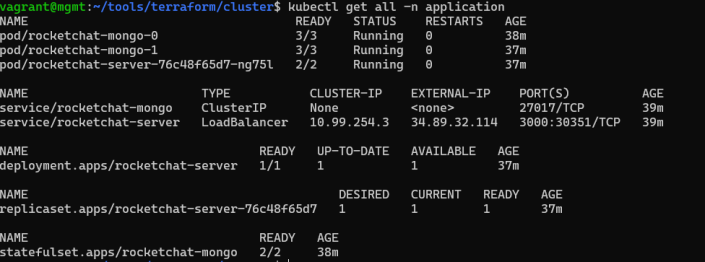
\includegraphics[width=1.0\textwidth]{./pictures/kubctl-get-all-application-ns.png}
    \caption{All resources from application namespace}
    \label{fig:all-resources-application-namespace}
\end{figure}

In a briefly way, it is possible to see that what was deployed was (more information in Analysis Section \ref{section:analysis}):
\begin{itemize}
    \item RocketChat Pods to handle the requests from the client (RocketChat servers).
    \item RocketChat Service to load-balance the client requests for the RocketChat Pods.
    \item MongoDB Pods to handle the requests from RocketChat servers (are the pods called RocketChat-Mongo).
    \item MongoDB Service to be forward the traffic to MongoDB Pods.
\end{itemize}

Second, let's get all resources related to the application namespace running the command \textit{kubectl get all -n istio-system} producing the output in the Figure \ref{fig:all-resources-istio-namespace}.

\begin{figure}[h]
    \centering
    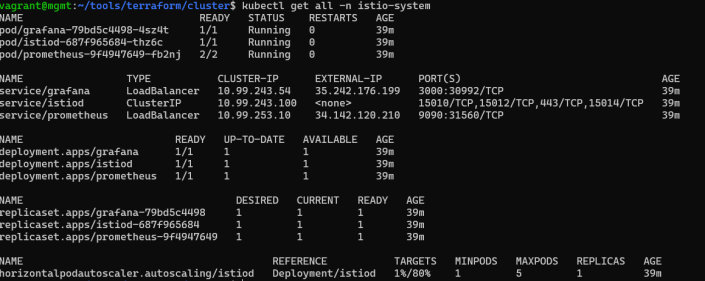
\includegraphics[width=1.0\textwidth]{./pictures/kubctl-get-all-istio-system-ns.png}
    \caption{All resources from istio-system namespace}
    \label{fig:all-resources-istio-namespace}
\end{figure}

In a briefly way, it is possible to see that what was deployed was (more information in Analysis Section \ref{section:analysis}):
\begin{itemize}
    \item Grafana Pods to handle the requests for monitoring purposes.
    \item Grafana Service to load-balance the client requests for Grafana Pods.
    \item Prometheus Pods that collect metrics about the cluster and its resources.
    \item Prometheus Service to load-balance the client requests for the Prometheus Pods.
\end{itemize}

After the deployment, if it is needed to use the tool \textit{kubectl} for any purpose, first it is needed to run the following command, changing the parameters with anchors($<$parameter$>$) with the respective project data:
\begin{lstlisting} [style=Bash]
vagrant@mgmt:~/tools/terraform/cluster$ gcloud container clusters get-credentials <project_name> --zone <project_zone>
\end{lstlisting}

\section{Notes}
\begin{itemize}
    \item If it is needed more worker nodes, it is possible to do it by changing the \textit{workers\_count} variable in the file \textit{terraform.tfvars}.
    \item If it is needed more replicas of the RocketChat-server or RocketChat-mongo, it is possible to do it by changing the \textit{replicas} variable in the file \textit{k8s-pods.tf}. For grafana and prometheus the same variable should be change in their respective .yml file inside the monitoring folder. If the cluster is already running it can also be added replicas using the kubernetes command line tool.
    \item If it is needed to change the region, it is possible to do it by changing the \textit{region} variable in the file \textit{terraform.tfvars}.
    \item Currently there is a bug by the application's development team that prevents the rocket-chat's setup-wizard from working as intended but that is outside the scope of our work. The problem is in the developer team of RocketChat, because there is full connectivity between the respective resources of the cluster. As we can in \ref{fig:html-from-rocektchar-pod} see rocketchat-server service responds perfectly well to a client request. If that didn't happen, an 50X error would be given.
\end{itemize}

\begin{figure}[h]
    \centering
    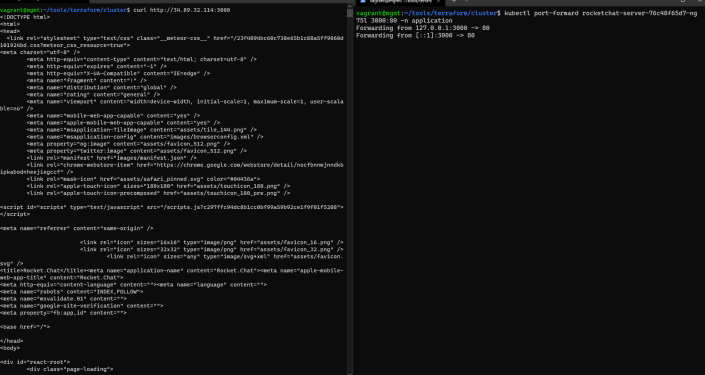
\includegraphics[width=1.0\textwidth]{./pictures/curl-success-page-rocketchat.png}
    \caption{Portforwarding to the RocketChat Pod and Curl command to get the RocketChat page directly from the Pod is successful}
    \label{fig:html-from-rocektchar-pod}
\end{figure}

% #############################################################################
\cleardoublepage
% #############################################################################
\chapter{Versioning}
\label{chapter:versioning}
For this project, the RNL Git (\url{https://git.rnl.tecnico.ulisboa.pt/AGISIT-21-22/team-06}) was used for versioning.

\cleardoublepage
% #############################################################################
\chapter{Work Evolution}
\label{chapter:work-evol}

With this project was possible to show an example on how to deploy and provision tiered Microservices-based containerized Web Application on a Public Cloud using automation tools as well as implementing instrumentation on the applications, services and infrastructure components of the solution, to allow monitoring and logging features. 

Initially, the system was deployed using the following tools: Terraform to create the infrastructure, Ansible to configure the infrastructure created and then Docker Compose to deploy the services needed. This version is called Docker Compose Version. \textbf{The goal for this project was to try several tools and learn as much as possible} and that is the reason why the Docker Compose was chosen over Kubernetes as first hand. With the Docker Compose, some limitations were found. The first limitation is that it was needed more files and commands to run the application because the method used is more manual. With Docker Compose it is possible to configure and start multiple Docker containers on the same host so, it was needed multiple commands Docker Compose to deploy the services needed on each host (There was a host for RocketChat, another for Mongo, one more for Grafana, and another one for Prometheus - as can be seen in the Figure \ref{fig:docker-compose-version-proj-struc} which shows the project structure of the Docker Compose Version). The second limitation found resides in the fact that the scaling up/down mechanism of Docker Compose is also "kinda" manual because it is needed to run a command each time some scaling is needed (for example, running the docker-compose command with the flag \textit{--scale serviceX=5} which would increase the serviceX number of containers to 5). 

\begin{figure}[h]
    \centering
    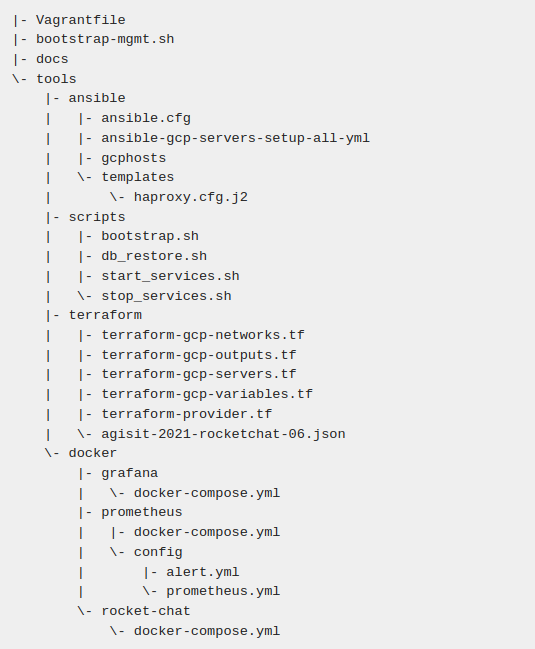
\includegraphics[width=0.8\textwidth]{./pictures/docker-compose-version-proj-structure.png}
    \caption{Docker Compose Version Project Structure}
    \label{fig:docker-compose-version-proj-struc}
\end{figure}

After analysing the limitations, the group chose to change the orchestration tool for \ac{K8s} for a better reliable and automated solution. Although more complex, \ac{K8s} gives more flexibility and the possibility of making an Autoscalable System (scaling mechanism can be automatic compared to the scaling mechanism of Docker Compose). Also, in the final solution the deployment process is now faster and more autonomous.

%\lipsum[61-63]
% #############################################################################
%                        END OF MAIN DOCUMENT BODY
% #############################################################################
% -----------------------------------------------------------------------------
%  Bibliography
% -----------------------------------------------------------------------------
%\bibliographystyle{IEEEtran}
% > entries ordered in the order in which the citations appear, with numeric 
% reference markers
% External bibliography database file in the BibTeX format
\cleardoublepage
%\bibliography{IST-UL-Project-Report_bib_DB}
\begin{thebibliography}{9}
% Add entry in the table of contents as chapter
\addcontentsline{toc}{chapter}{\bibname}

\bibitem{rocketchat}
RocketChat. \url{https://rocket.chat/}

\bibitem{mongodb}
MongoDB. \url{https://en.wikipedia.org/wiki/MongoDB}

\bibitem {grafana}
Grafana. \url{https://en.wikipedia.org/wiki/Grafana}

\bibitem{prometheus}
Prometheus. \url{https://en.wikipedia.org/wiki/Prometheus_(software)}

\bibitem {rocketchat-create-docker-container}
RocketChat. High Availability. Create rocket.chat docker container. \url{https://docs.rocket.chat/quick-start/installing-and-updating/docker-containers/high-availability-install#create-rocket.chat-docker-container}

\bibitem{running-mongodb-on-kubernetes}
Running MongoDB on Kubernetes with StatefulSets. (2017, Jan 30). Document Website: \url{https://kubernetes.io/blog/2017/01/running-mongodb-on-kubernetes-with-statefulsets/}

\end{thebibliography}
% #############################################################################
\end{document}
% #############################################################################

